\documentclass{beamer}
\usepackage[utf8]{inputenc}
\usepackage[]{amsmath}
\usepackage{graphicx}
\usepackage{physics}
\usepackage{subcaption} % package pour faire des subfigures
\usepackage{multirow} % package pour multirow/multicolumn
\usepackage{booktabs} % package pour top/mid/bottom rule
\usepackage{tcolorbox} % toujours plus de boites
\usepackage{tabularx}
%\usepackage[backend=biber]{biblatex}
%
%
%\addbibresource{Biblio_dbl_quantum.bib}

%\bibliographystyle{stylename}
%\bibliography{Biblio_dbl_quantum}

\title{Cross-relaxation in dense ensembles of NV centers and
application to magnetometry}
\author{Clément Pellet-Mary}
\date{PhD Defense}

\mode<presentation> {\usetheme{Rochester}}

\begin{document}
\begin{frame}
\maketitle
%\begin{center}
%\includegraphics[width=\textwidth,height=0.3\textheight,keepaspectratio]{logos}
%\end{center}
\end{frame}

\begin{frame}{Outline}
\tableofcontents
\end{frame}

\section{Sensing with quantum mechanics}
\begin{frame}{Outline}
\tableofcontents[currentsection]
\end{frame}

\begin{frame}{Quantum sensing and metrology}
\centering
\includegraphics[width=\textwidth,height=0.9\textheight,keepaspectratio]{Slide_quantum_metrology}
\end{frame}

\begin{frame}{Magnetometry applications}
\centering
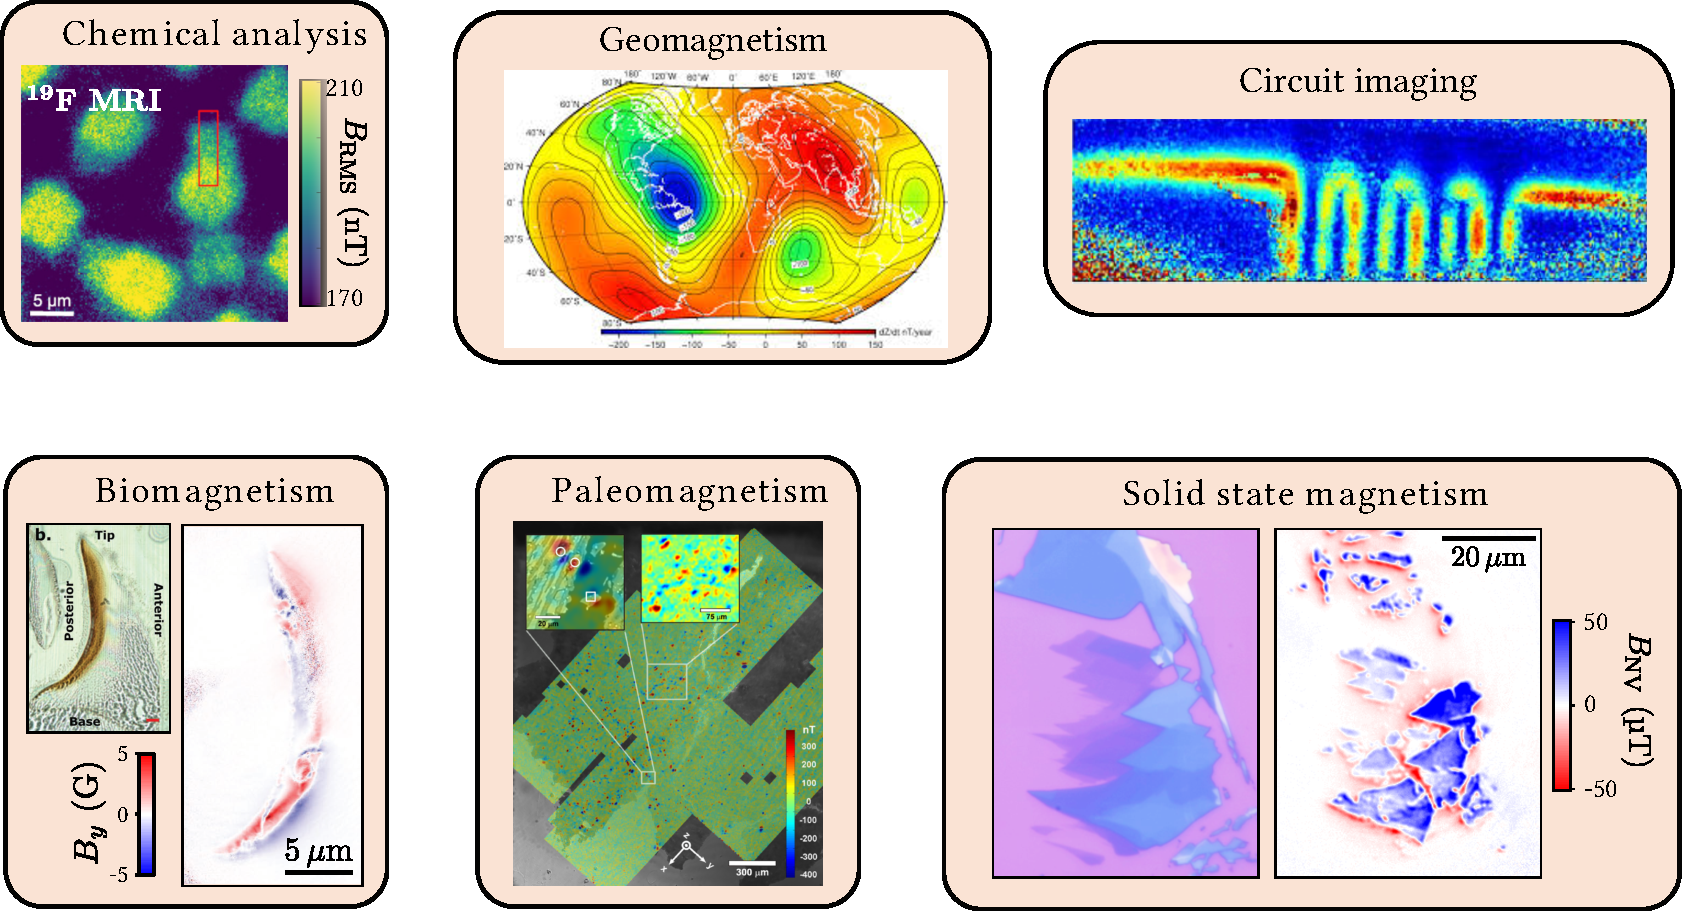
\includegraphics[width=\textwidth,height=0.9\textheight,keepaspectratio]{Slide_example_magnetometry}
\end{frame}

\begin{frame}{Quantum magnetometers}
\centering
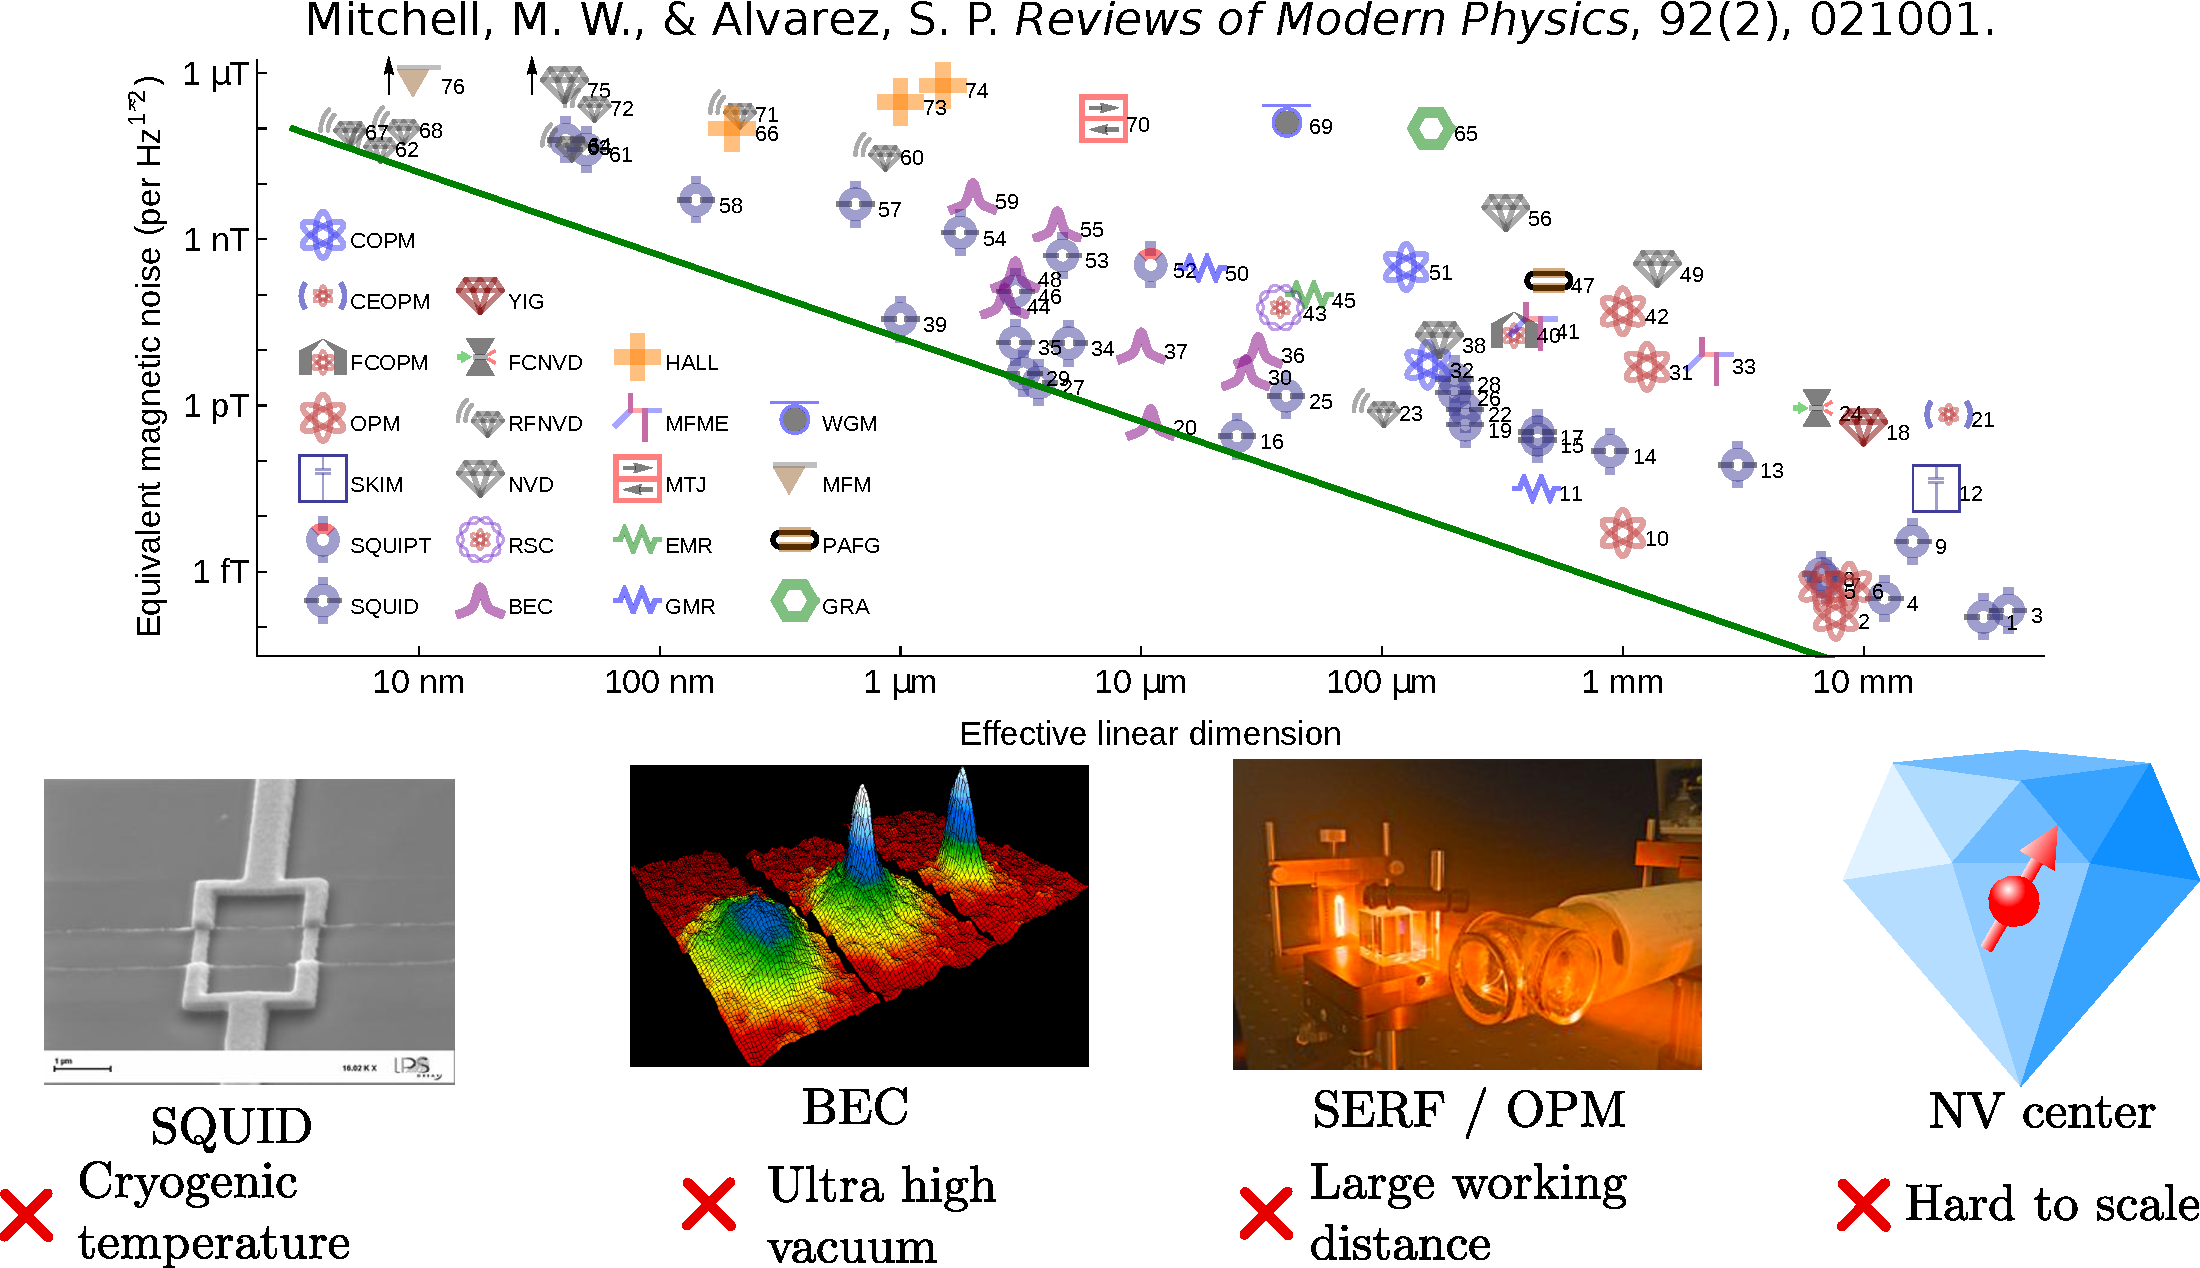
\includegraphics[width=\textwidth,height=0.9\textheight,keepaspectratio]{Slide_quantum_magnetometers}
\end{frame}

\section{Magnetometry with NV centers}
\begin{frame}{Outline}
\tableofcontents[currentsection]
\end{frame}

\begin{frame}{Colored centers in diamond}
\centering
\includegraphics[width=\textwidth,height=0.9\textheight,keepaspectratio]{Slide diamant}
\end{frame}

\begin{frame}{Synthetic diamond and NV centers}
\centering
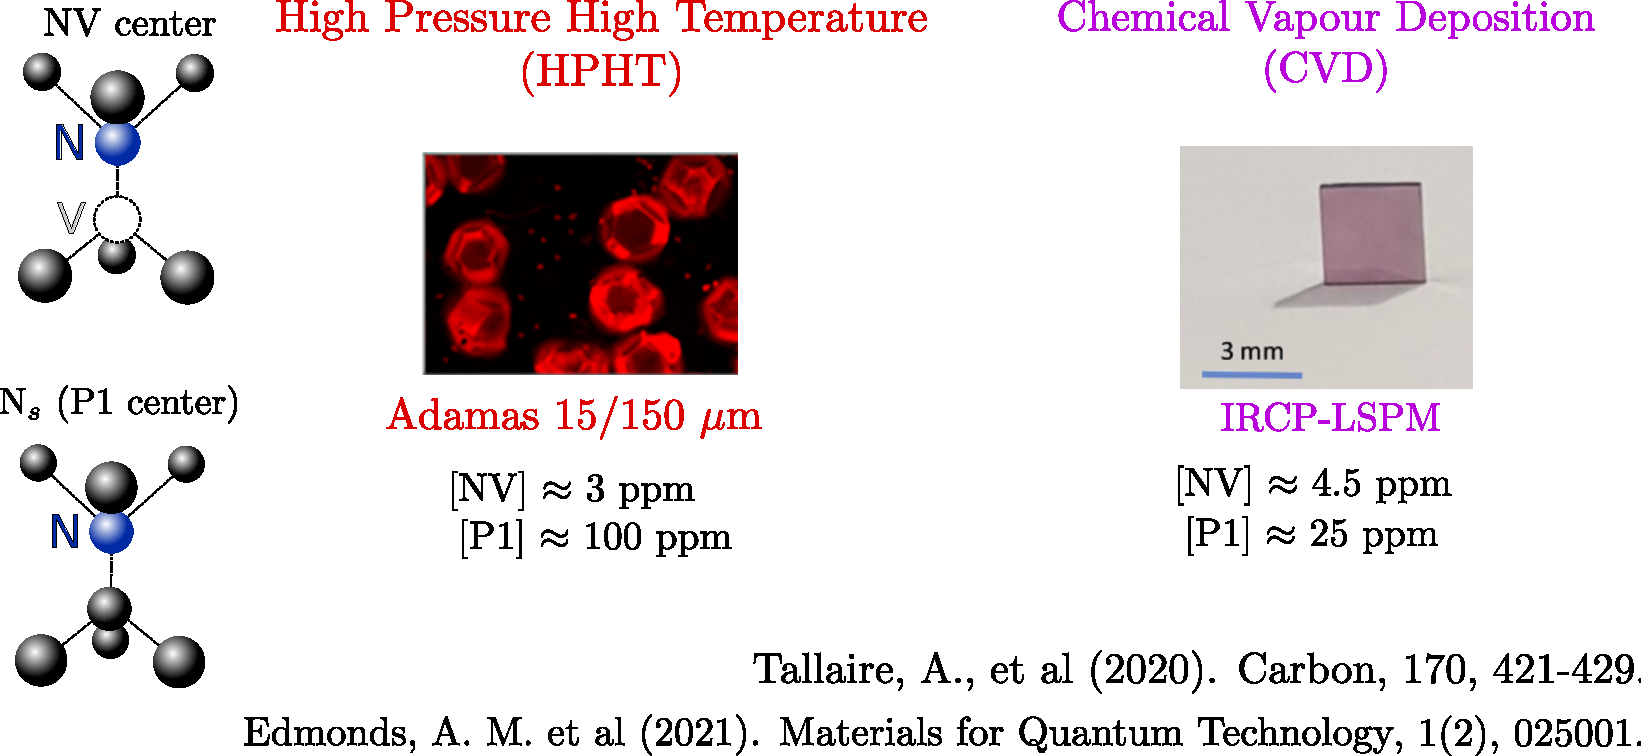
\includegraphics[width=\textwidth,height=0.9\textheight,keepaspectratio]{Slide_fab_sample}
\end{frame}

\begin{frame}{The NV center energy levels}
\centering
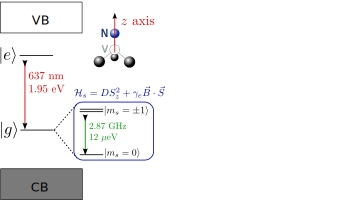
\includegraphics[width=\textwidth,height=0.9\textheight,keepaspectratio]{Slide_NV_levels_1}
\end{frame}

\begin{frame}{The NV center energy levels}
\centering
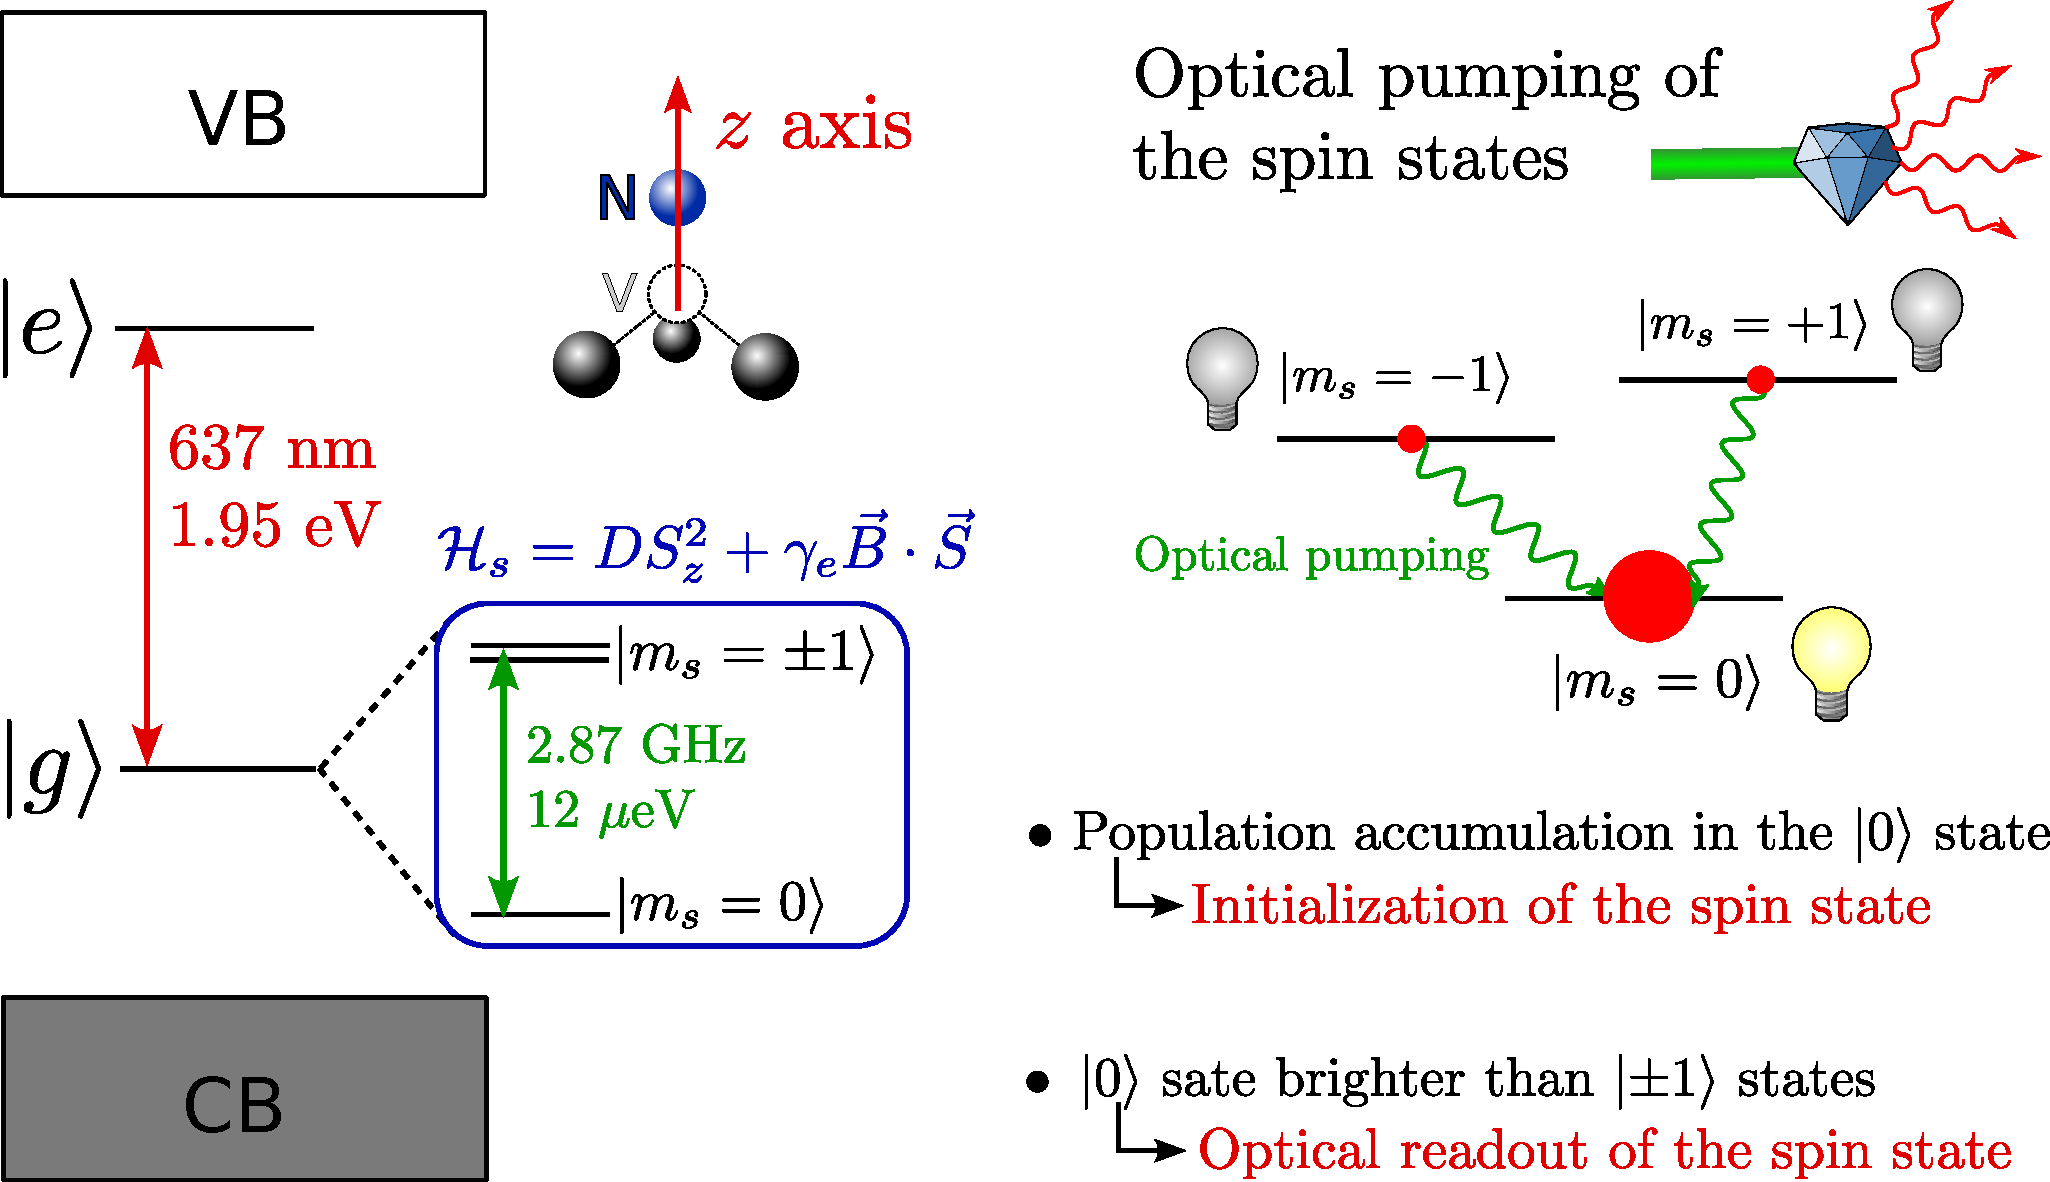
\includegraphics[width=\textwidth,height=0.9\textheight,keepaspectratio]{Slide_NV_levels}
\end{frame}

\begin{frame}{Optically detected magnetic resonance (ODMR)}
\centering
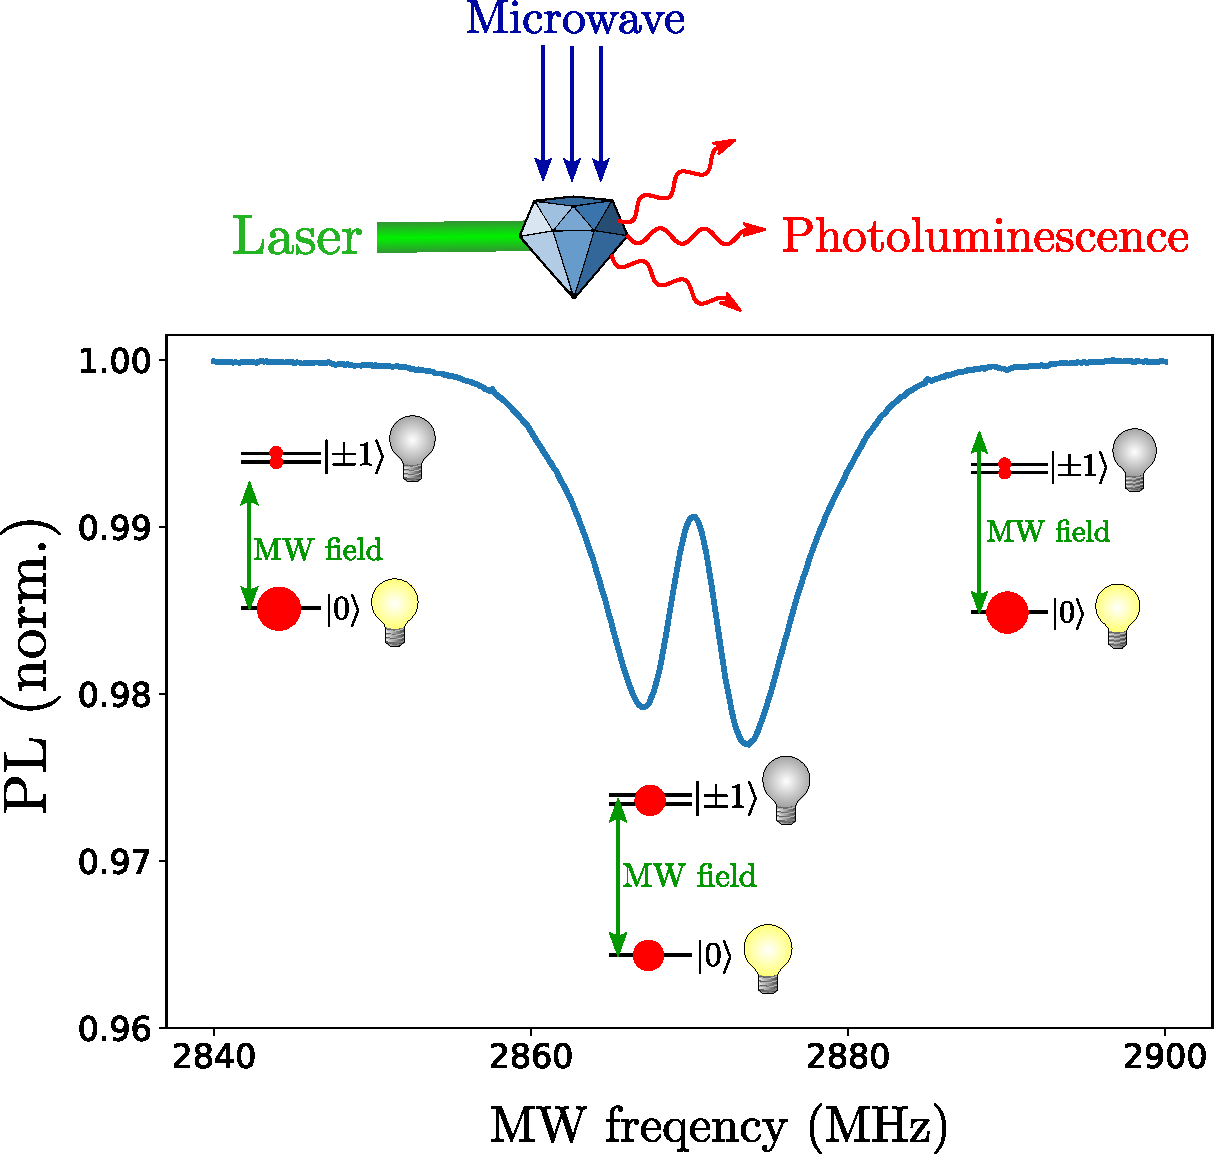
\includegraphics[width=\textwidth,height=0.9\textheight,keepaspectratio]{Slide_ODMR_0}
\end{frame}

\begin{frame}{Experimental setup}
\centering
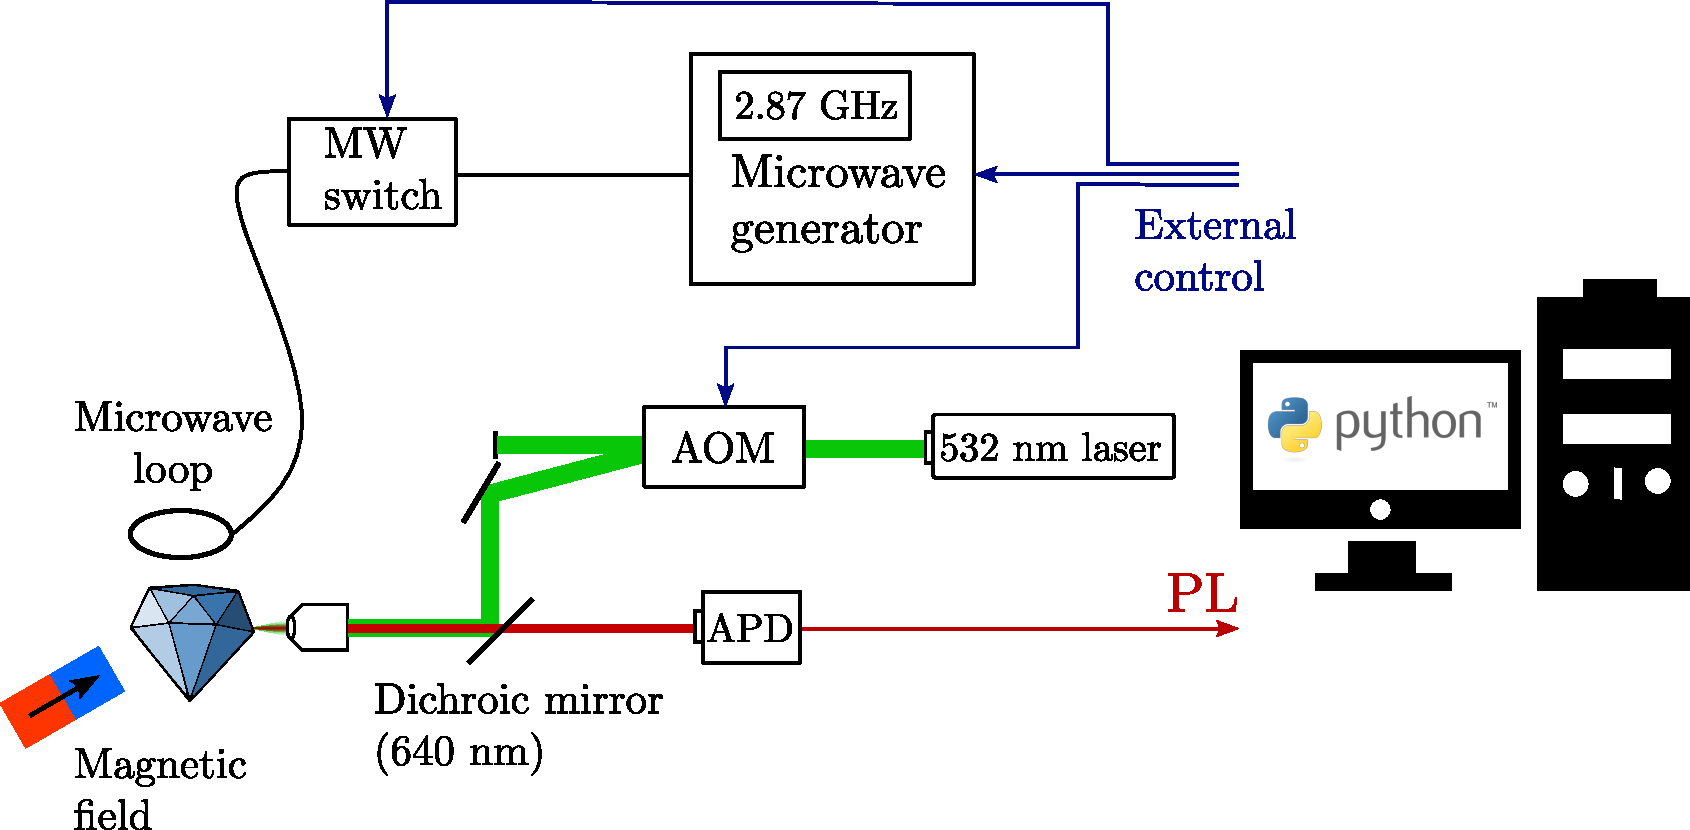
\includegraphics[width=0.9\textwidth,height=0.9\textheight,keepaspectratio]{Slide_setup}
\end{frame}

\begin{frame}{ODMR with NV ensemble}
\centering
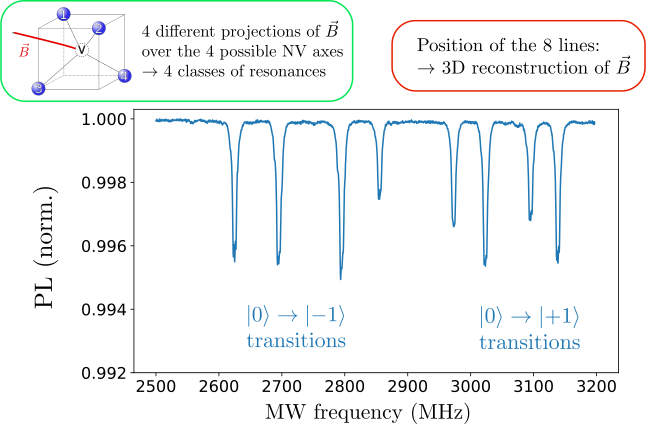
\includegraphics[width=\textwidth,height=0.9\textheight,keepaspectratio]{Slide_ODMR_8_classes}
\end{frame}

\begin{frame}{Sensitivity limit for NV ensemble magnetometry}
\centering
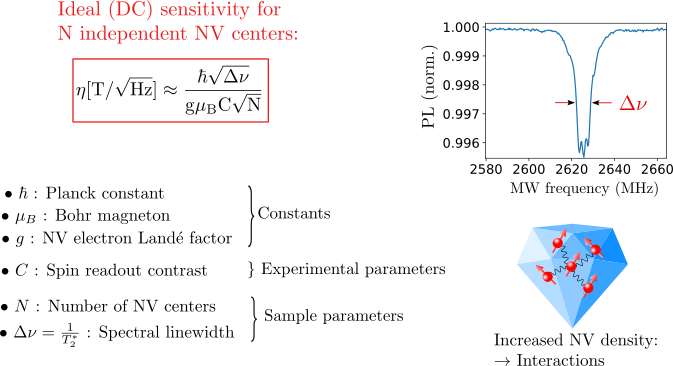
\includegraphics[width=\textwidth,height=0.9\textheight,keepaspectratio]{Slide_NV_ensemble_sensi}
\end{frame}

\begin{frame}{Dipole-dipole interaction between two electronic spins}
\centering
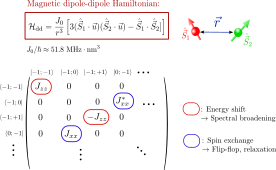
\includegraphics[width=\textwidth,height=0.9\textheight,keepaspectratio]{Slide_dipole_dipole}
\end{frame}

\begin{frame}{Interaction limit to NV ensemble magnetometry}
\centering
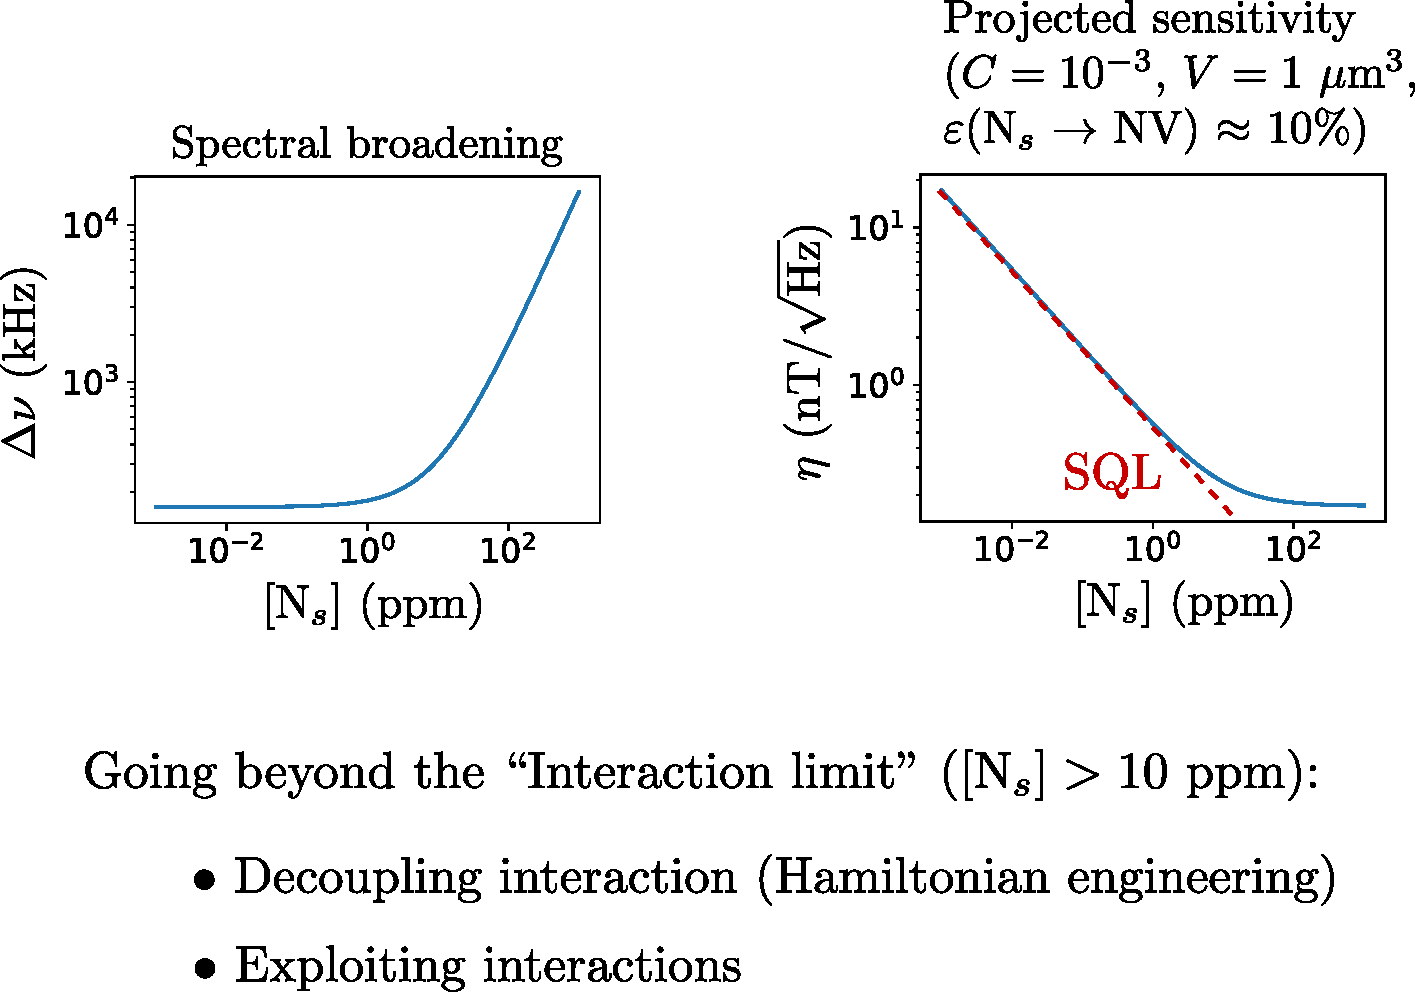
\includegraphics[width=\textwidth,height=0.9\textheight,keepaspectratio]{Slide_interaction_limit}
\end{frame}



\section{Low field depolarization magnetometry (LFDM)}
\begin{frame}{Outline}
\tableofcontents[currentsection]
\end{frame}

\begin{frame}{Depolarization of dense NV ensemble at low magnetic field}
\centering
\includegraphics[width=\textwidth,height=0.9\textheight,keepaspectratio]{slide_presentation_sujet}
\end{frame}

\begin{frame}{Pesentation of low field depolarization magnetometry (LFDM)}
\centering
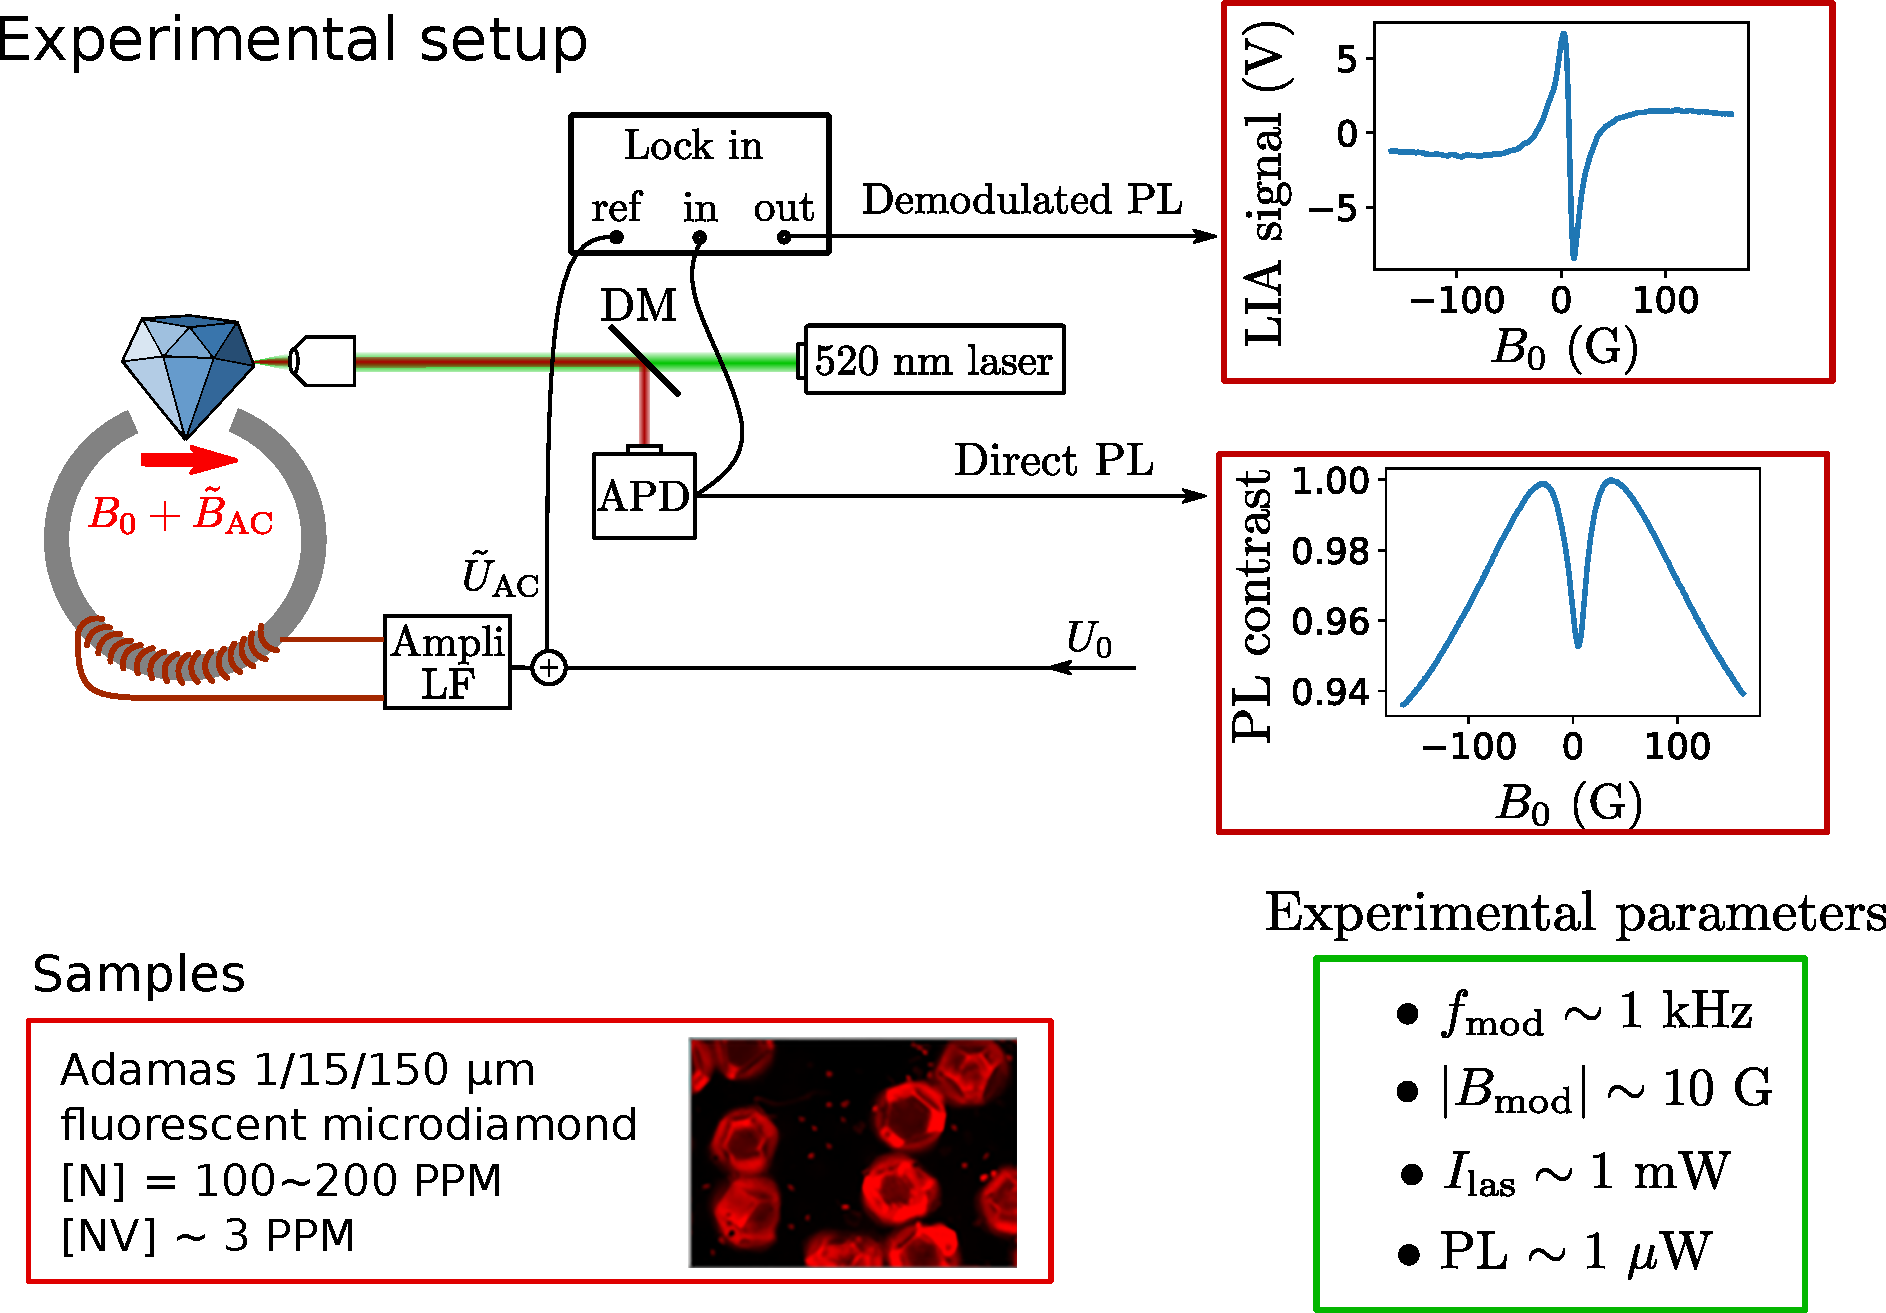
\includegraphics[width=\textwidth,height=0.9\textheight,keepaspectratio]{Slide_principle_LFDM}
\end{frame}

\begin{frame}{Sensitivity of LFDM}
\centering
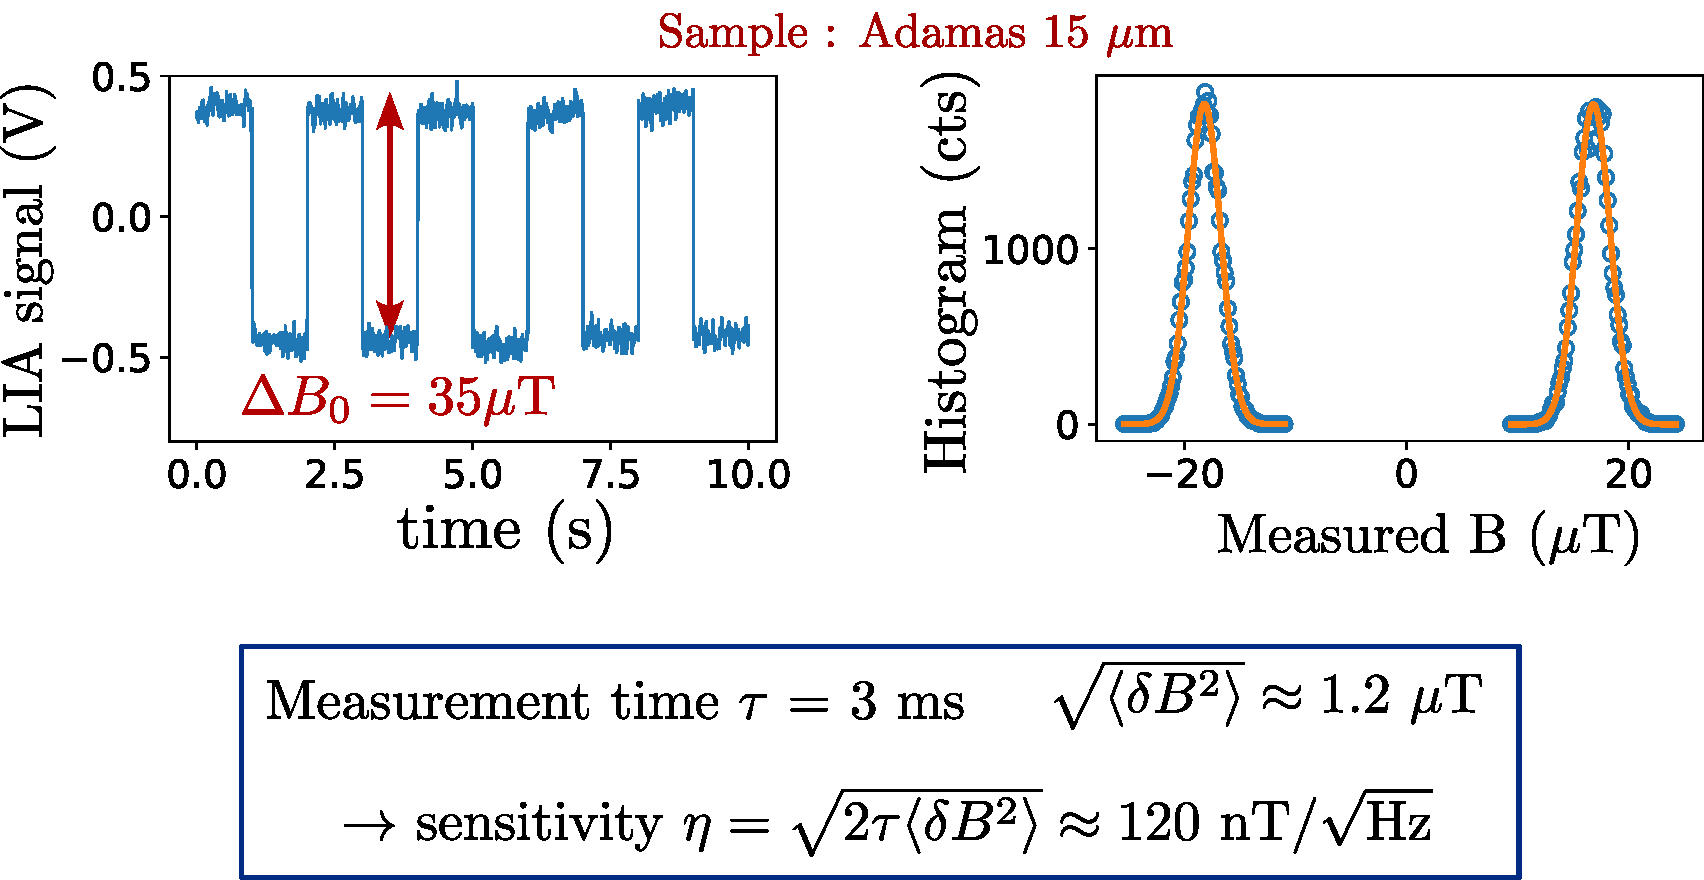
\includegraphics[width=\textwidth,height=0.9\textheight,keepaspectratio]{Slide_sensi_LFDM}
\end{frame}

\begin{frame}{Comparison with the state of the art}
\centering
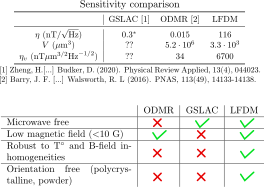
\includegraphics[width=\textwidth,height=0.9\textheight,keepaspectratio]{Slide_comparison_litterature}
\end{frame}

\begin{frame}{Comparison with CW ODMR}
\centering
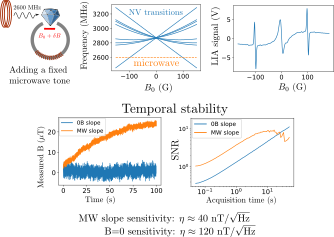
\includegraphics[width=\textwidth,height=0.9\textheight,keepaspectratio]{Slide_comparison_microwave}
\end{frame}

\begin{frame}{Application: wide-field magnetometry on irregular surfaces}
\centering
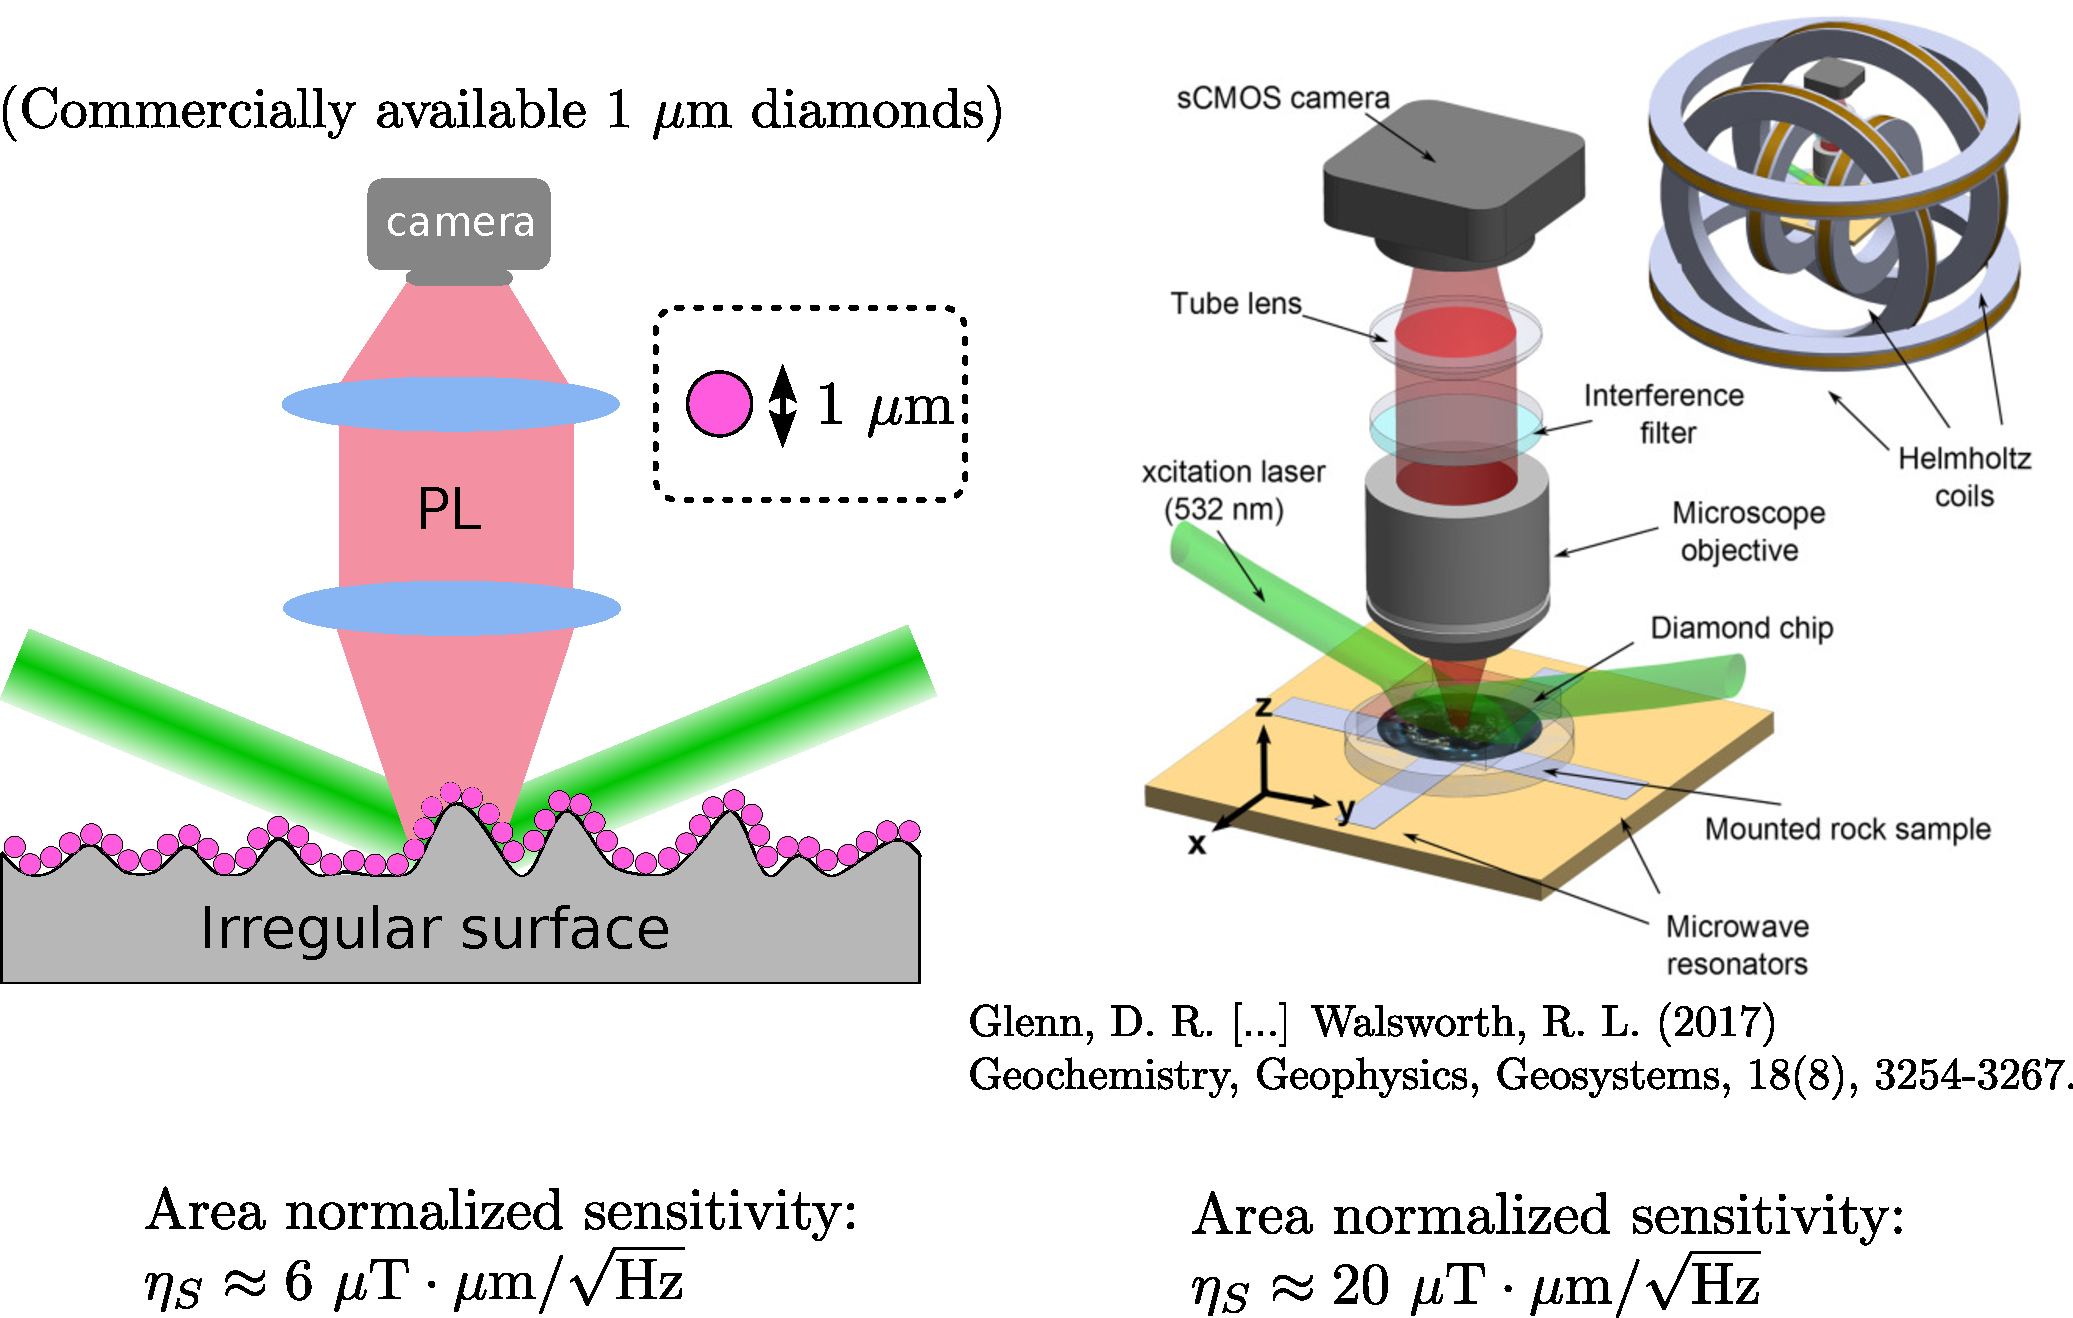
\includegraphics[width=\textwidth,height=0.9\textheight,keepaspectratio]{Slide_applications_wide_field}
\end{frame}

\section{Depolarization mechanisms in dense NV ensemble}
\begin{frame}{Outline}
\tableofcontents[currentsection]
\end{frame}
\begin{frame}{Principle of cross-relaxation with NV centers}
\centering
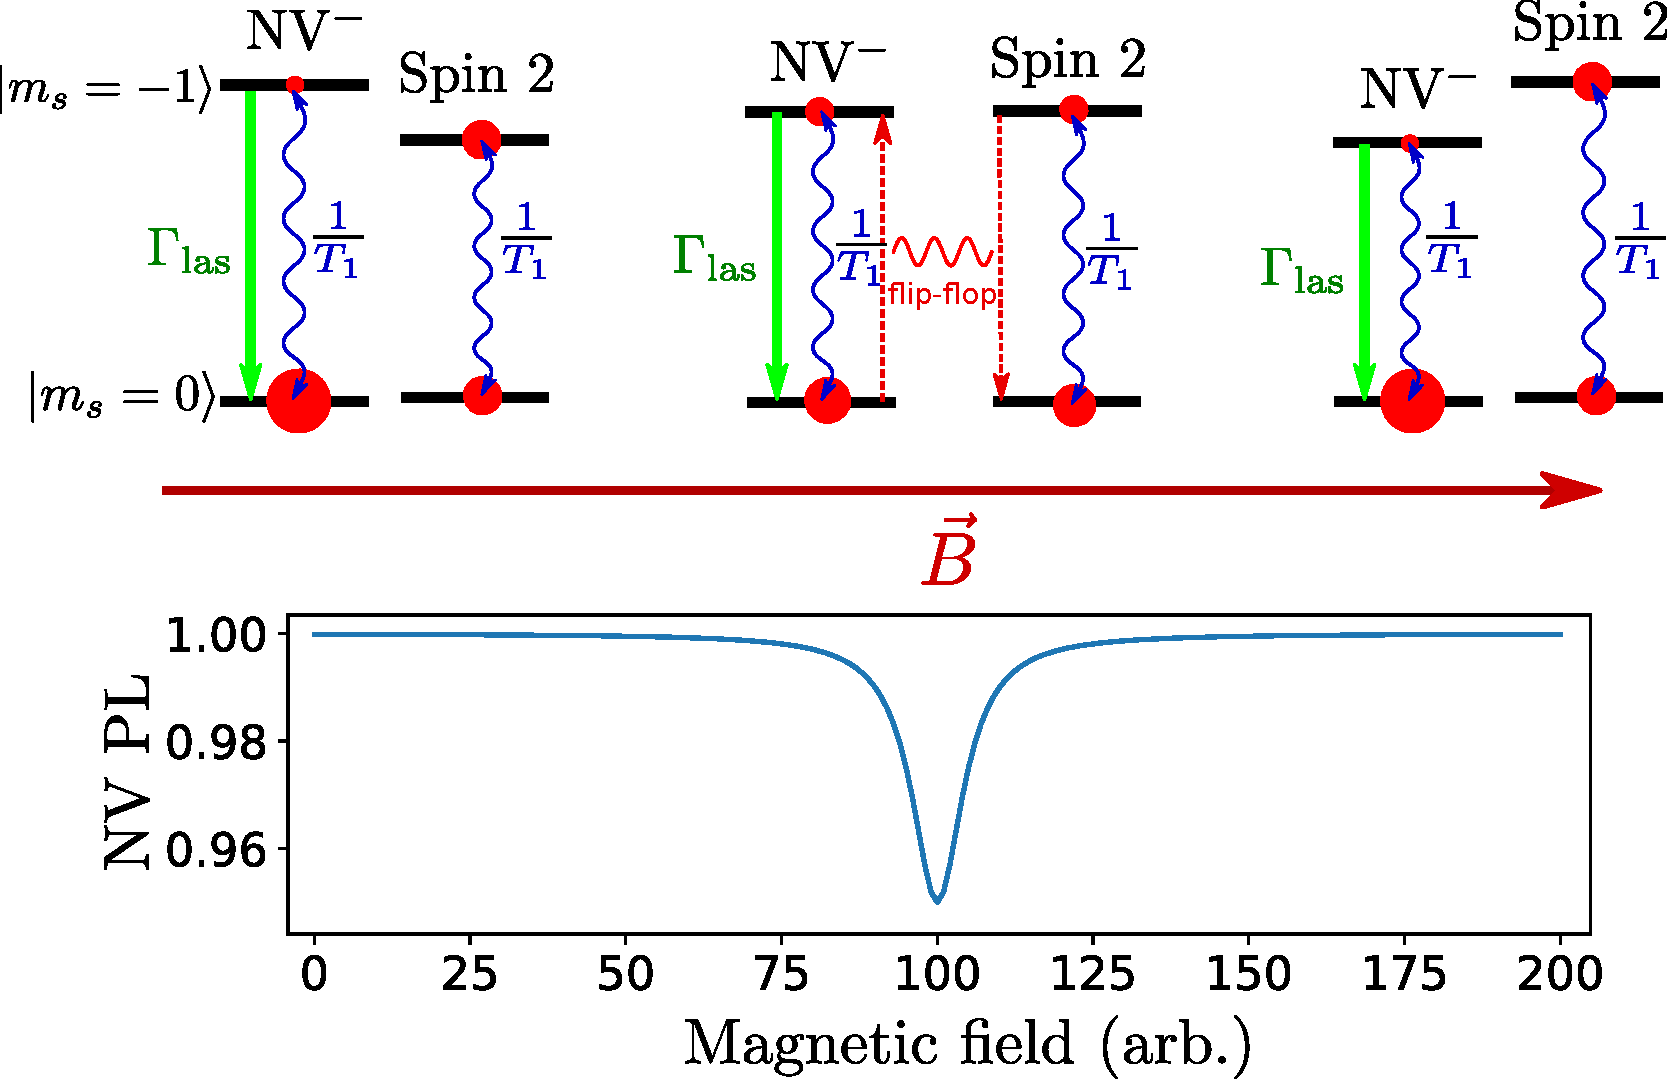
\includegraphics[width=\textwidth,height=0.8\textheight,keepaspectratio]{Slide_CR_presentation}
\end{frame}

\begin{frame}{Example: Cross-relaxation between NV centers and VH$^-$}
\centering
\includegraphics[width=\textwidth,height=0.9\textheight,keepaspectratio]{Slide_CR_VH}
\end{frame}

\begin{frame}{Cross-relaxation between NV centers and NV centers}
\centering
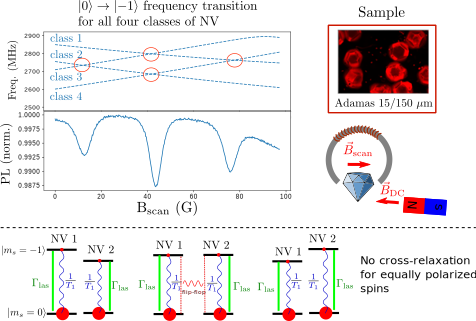
\includegraphics[width=\textwidth,height=0.9\textheight,keepaspectratio]{Slide_CR_adamas}
\end{frame}

\begin{frame}{Presentation of the fluctuator model}
\centering
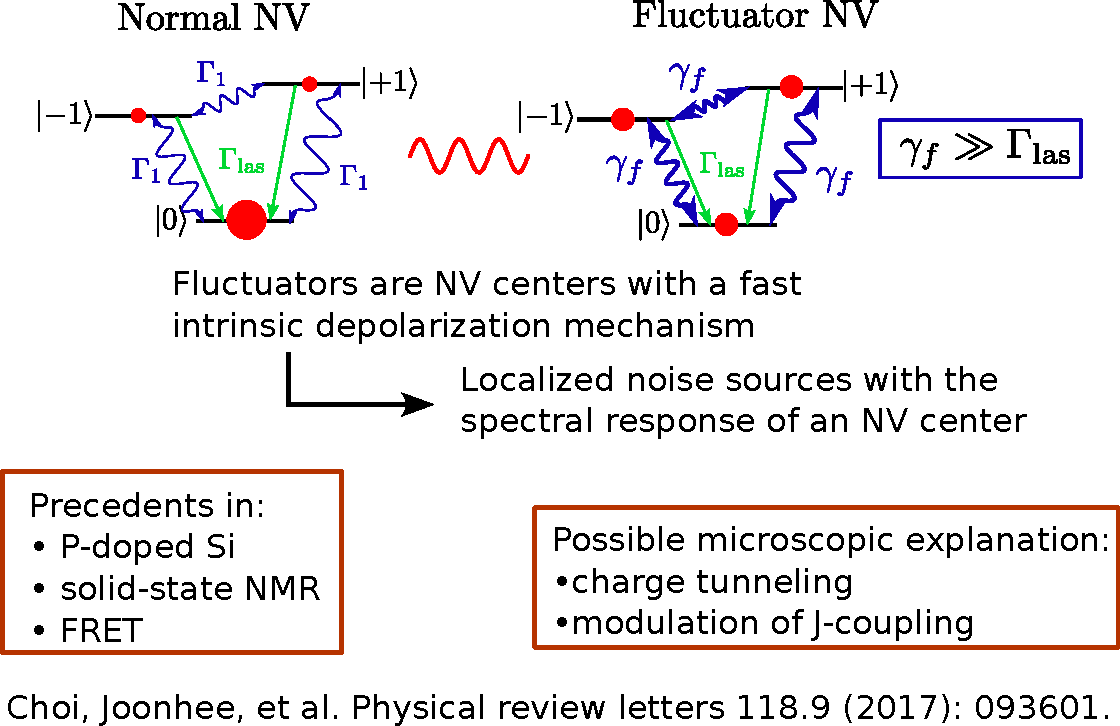
\includegraphics[width=\textwidth,height=0.8\textheight,keepaspectratio]{Slide_fluct_intro}
\end{frame}

\begin{frame}{Stretched exponential decay profile}
\centering
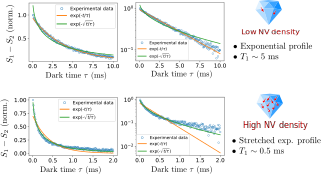
\includegraphics[width=\textwidth,height=0.9\textheight,keepaspectratio]{Slide_T1_exp_stretch}
\end{frame}

\begin{frame}{Zero field depolarization sources (theory)}
\centering
\includegraphics[width=\textwidth,height=0.9\textheight,keepaspectratio]{Slide_0B_theorie}
\end{frame}

\begin{frame}{Experiment: $\vec B$ in arbitrary direction}
\centering
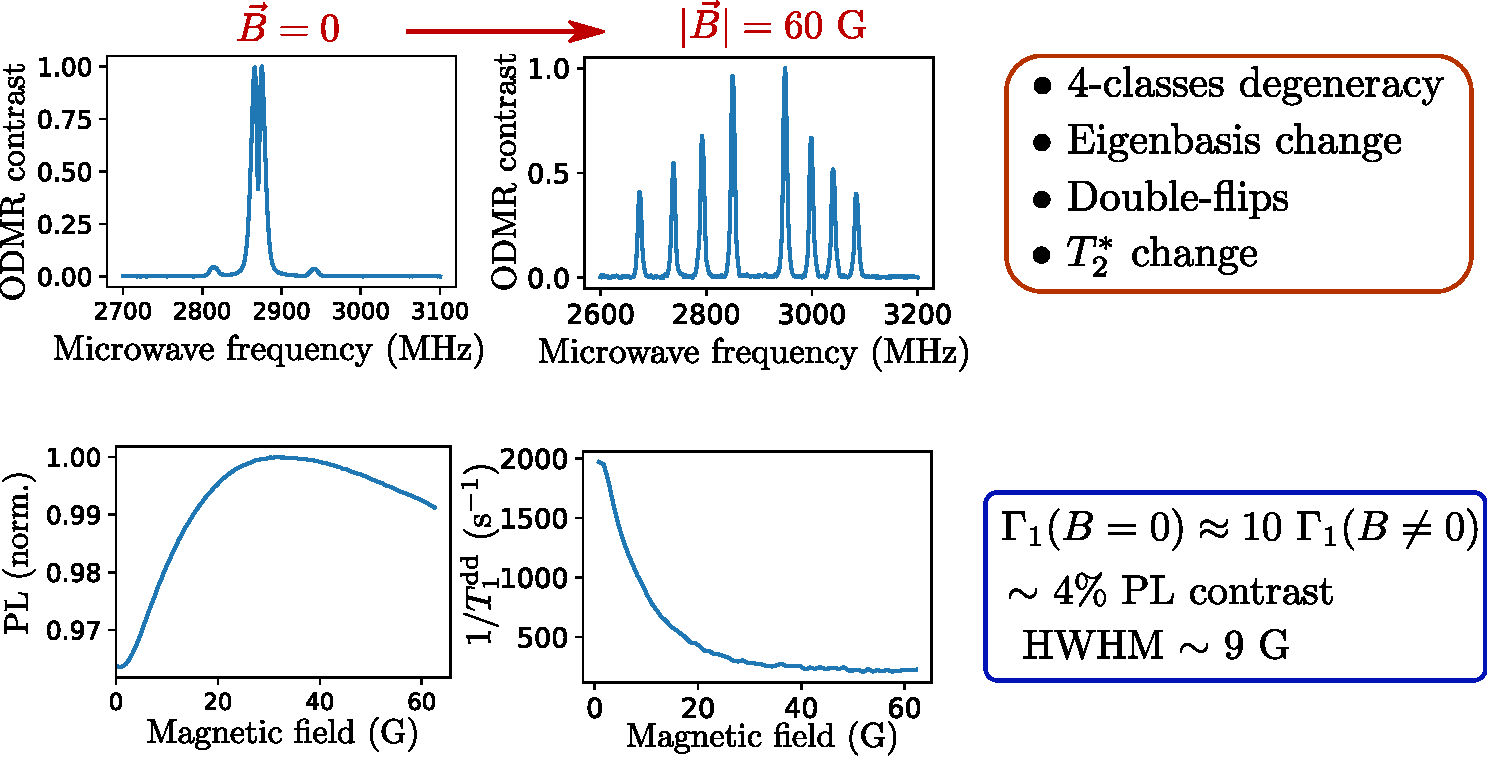
\includegraphics[width=\textwidth,height=0.9\textheight,keepaspectratio]{Slide_T1_PL_1x1x1x1}
\end{frame}

\begin{frame}{Experiment: $\vec B \parallel [100]$}
\centering
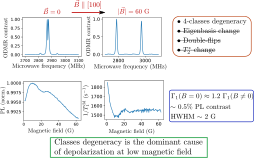
\includegraphics[width=\textwidth,height=0.9\textheight,keepaspectratio]{Slide_T1_PL_100}
\end{frame}

\begin{frame}{Experiment: $\vec B \perp [111]$}
\centering
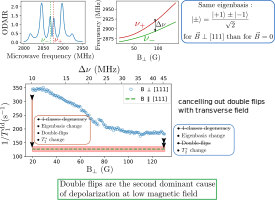
\includegraphics[width=\textwidth,height=0.9\textheight,keepaspectratio]{slide_champs_transverse}
\end{frame}

\begin{frame}{Summary of the experimental observations}
\centering
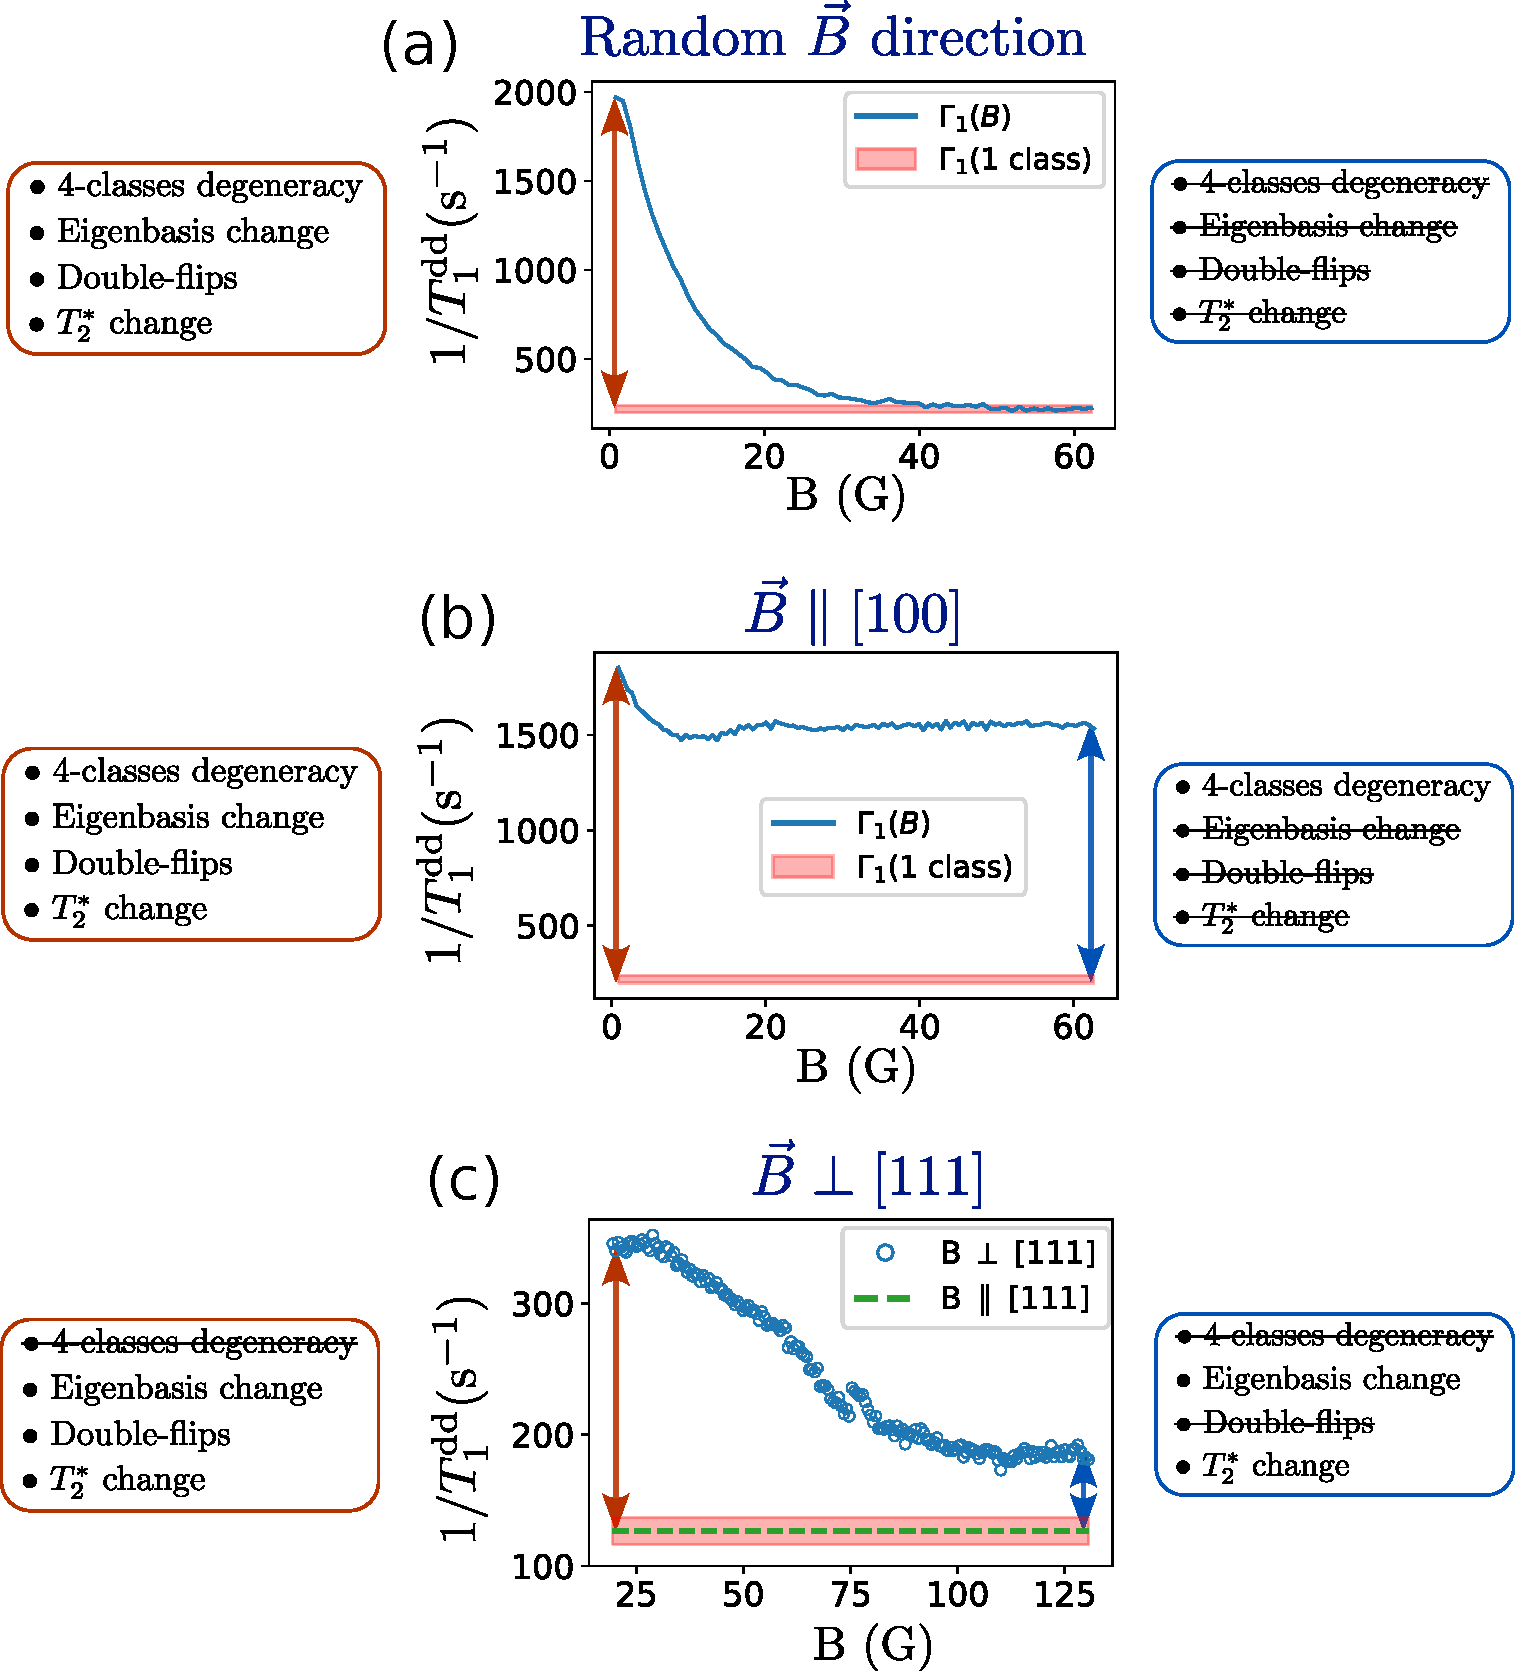
\includegraphics[width=\textwidth,height=0.9\textheight,keepaspectratio]{shema_summary_exp}
\end{frame}

\begin{frame}{Angular sensitivity of LFDM}
\centering
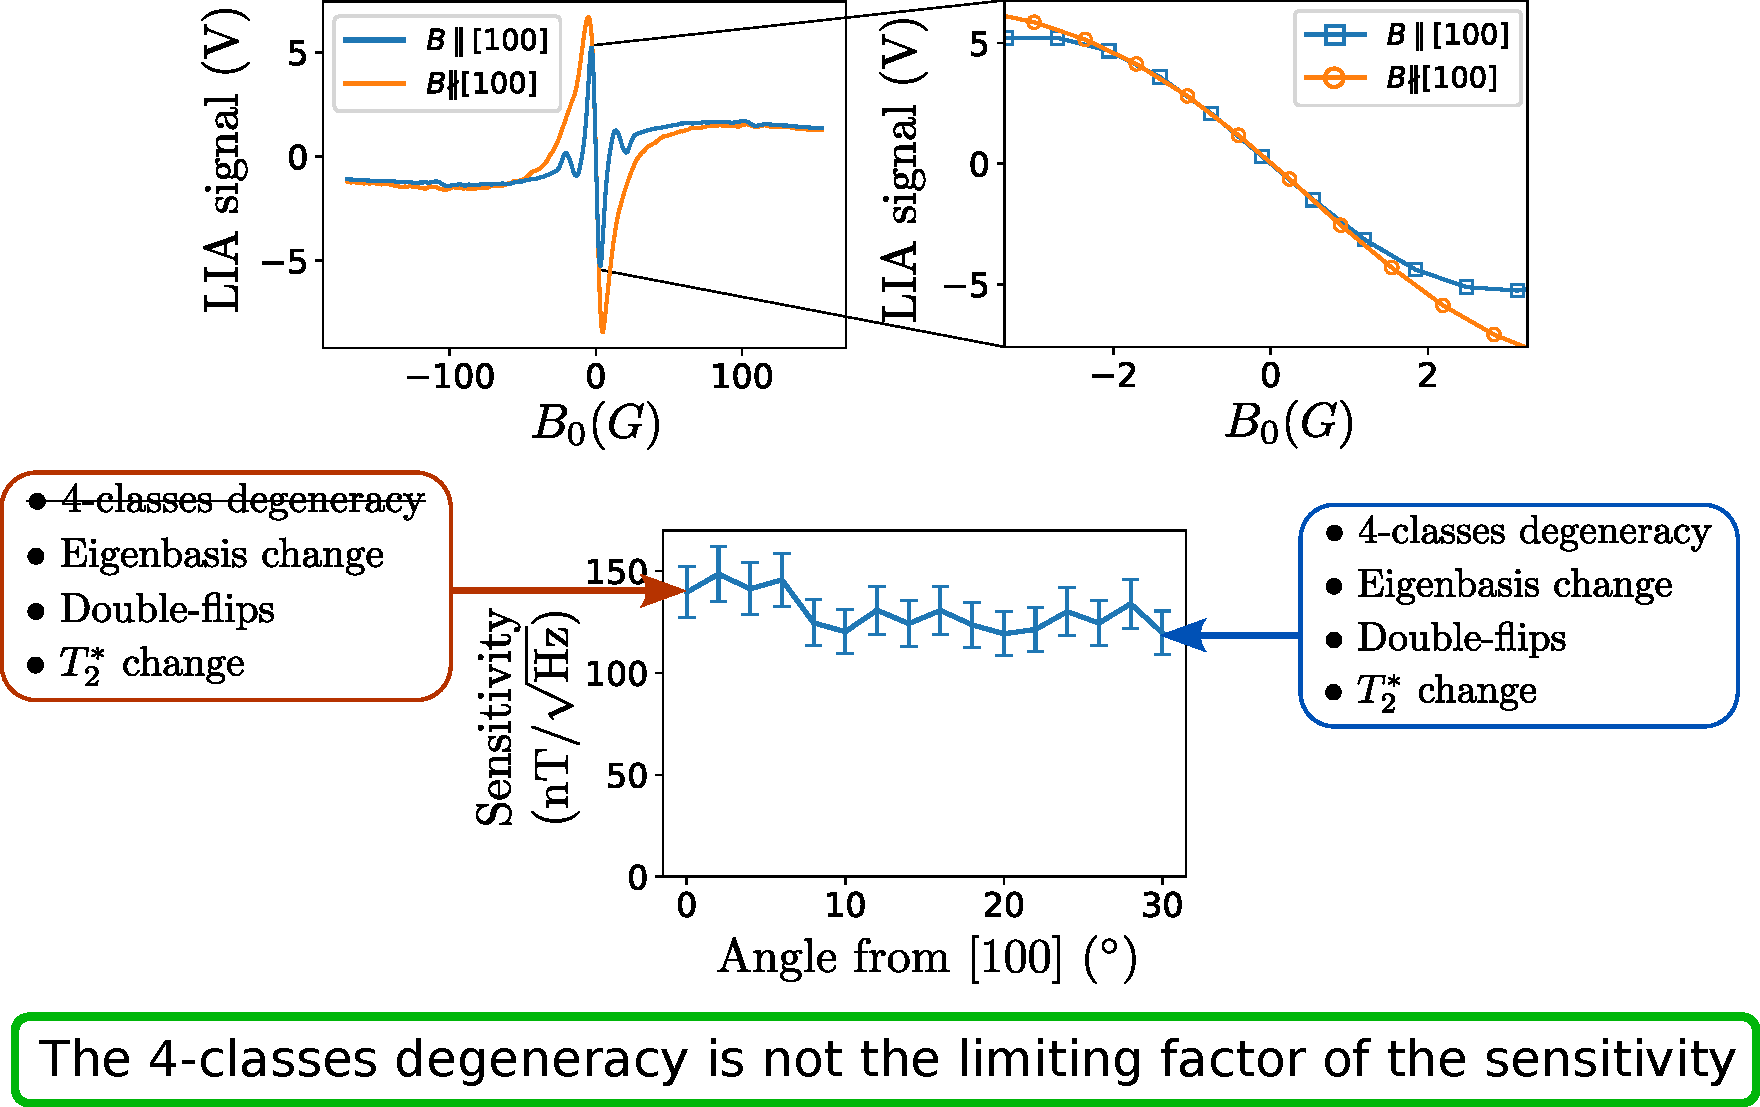
\includegraphics[width=\textwidth,height=0.9\textheight,keepaspectratio]{Slide_angular_sensitivity}
\end{frame}

\begin{frame}{Conclusion}

\end{frame}

\begin{frame}{Acknowledgments}

\end{frame}

\end{document}